\documentclass[10pt]{article}

\input{/Users/gabesekeres/Dropbox/LaTeX_Docs/pset_preamble.tex}

\course{ECON 6140}
\pset{4}
\begin{document}
\maketitle

\section*{Income Fluctuations Problem}

\begin{remark}
	Code is below, after the solutions to the Credit Markets problem. 
\end{remark}

Before writing the code, observe that the households solve the problem \[\max_{\{a_{t+1}c_t\}} \expect\barl \sum_{t=0}^\infty \beta^t \frac{c^{1-\gamma}}{1-\gamma}\barr \]subject to\begin{align*} c_t + a_{t+1} &= (1+r)a_t + y_t &&(\text{Budget Constraint}) \\ a_{t+1} &\ge -b &&(\text{Borrowing Constraint)}\\ \matrixc{\prob\{y_t = y_j \mid y_{t-1} = y_i\}}_{ij} &\equiv \matrixc{\pi_{HH} & \pi_{HL} \\ \pi_{LH} & \pi_{LL}}_{ij} &&(\text{Markov Process}) \end{align*}Following the strategy in QuantEcon, we will solve this using Euler Equation Time Iteration rather than Value Function Iteration. Formally, we have that the Euler Equation is \[c_t^{-\gamma} \le \beta (1+r) \expect \barl c_{t+1}^{-\gamma} \mid y_t\barr\]where this will hold with equality if and only if the borrowing constraint does not bind. Since income follows a (memoryless) Markov process, we look for time-invariant policy functions $a'(y,a)$ and $c(y,a)$ for savings and consumption respectively. Since utility is strictly increasing in consumption and CRRA utility function satisfy Inada, we can write $c(a,y) = (1+r)a + y - a'(a,y)$. Additionally, since the Euler Equation holding with equality (implying an interior solution) and the borrowing constraint binding are mutually exclusive, we can solve for the (functional) solution to the Euler Equation:\[\barl c(a,y)\barr^{-\gamma} = \beta (1+r) \sum_{y' \in \{y_H,y_L\}} \pi(y' \mid y) \barl c(a'(a,y),y')\barr^{-\gamma}\]and if the solution satisfies $a'(a,y) > -b$, we are done. Otherwise, we set $a'(a,y) = -b$ and solve for optimal consumption. With the structure defined, we can solve the problem computationally:

\begin{enumerate}
	\item I solved for the optimal consumption and savings policies when $r = 0.01$ and $b = 0$, using a tolerance of $1 \cdot 10^{-6}$. I achieved convergence in 145 iterations using a bisection algorithm. \newpage
	\item The optimal savings policy function is plotted in Figure~\ref{fig1}, and the optimal consumption policy function is plotted in Figure~\ref{fig2}. \begin{figure}[H] \centering 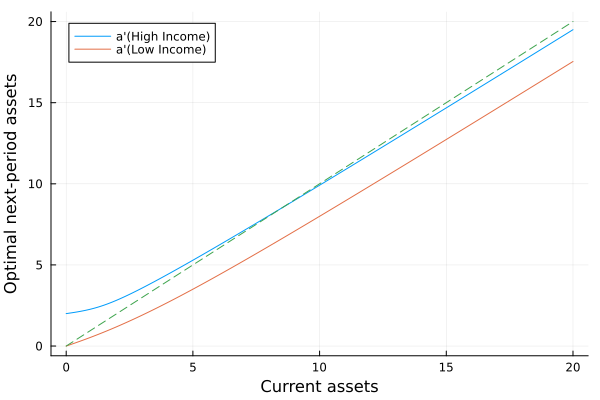
\includegraphics[width=10cm]{macro_hw4_code/savings_policy_function1.png}\caption{Optimal Savings Policy, $b = 0$}\label{fig1}\end{figure}\begin{figure}[H] \centering 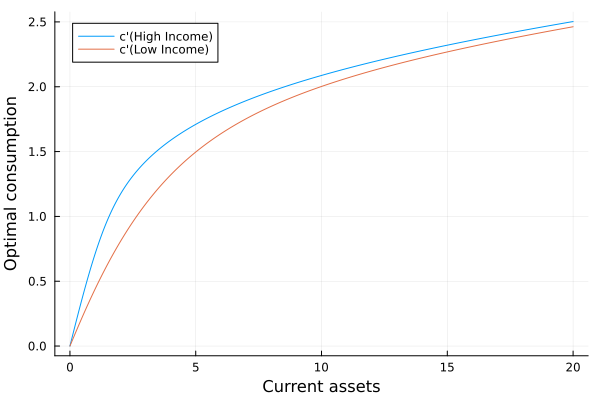
\includegraphics[width=10cm]{macro_hw4_code/consumption_policy_function1.png}\caption{Optimal Consumption Policy, $b=0$}\label{fig2}\end{figure} \newpage
	\item I increased the coefficient of relative risk aversion to 3, and plotted the new policies. I achieved convergence in 196 iterations. The results are Figure~\ref{fig3} and Figure~\ref{fig4}. As we can see, compared to the earlier plots the agent will consume less and save more when they are in the high-income state. As they are more risk-averse, they want to prevent the bad outcome -- less consumption when they have low-income -- more than in the previous question.\begin{figure}[H] \centering 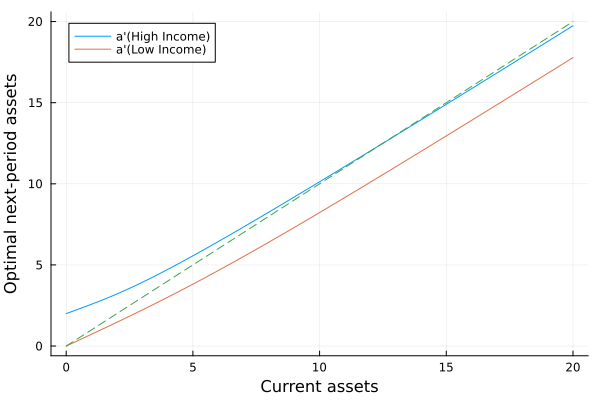
\includegraphics[width=10cm]{macro_hw4_code/savings_policy_function2.png}\caption{Optimal Savings Policy, $\gamma=3$}\label{fig3}\end{figure}\begin{figure}[H] \centering 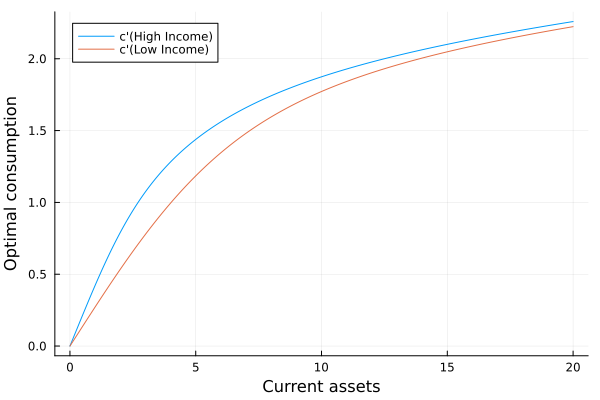
\includegraphics[width=10cm]{macro_hw4_code/consumption_policy_function2.png}\caption{Optimal Consumption Policy, $\gamma = 3$}\label{fig4}\end{figure}\newpage
	\item I set the borrowing constraint to $b = 4$, and solved for the new policies. I achieved convergence in 145 iterations. The results are Figure~\ref{fig5} and Figure~\ref{fig6}. As we can see, consumption increases and savings decrease in this model. This is because the households know that they can borrow if they end up in the bad state, and so are more willing to consume in the current period, especially when they have higher income. \begin{figure}[H] \centering 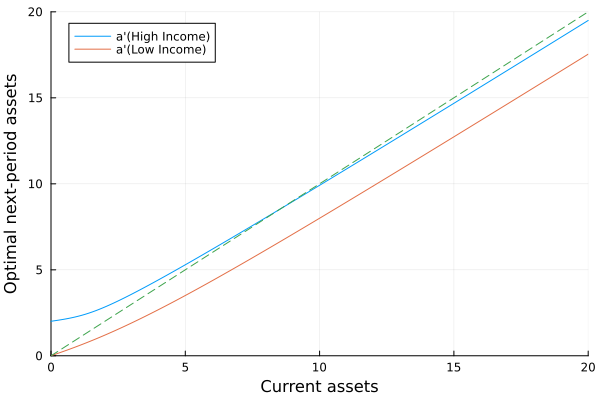
\includegraphics[width=10cm]{macro_hw4_code/savings_policy_function3.png}\caption{Optimal Savings Policy, $b=4$}\label{fig5}\end{figure}\begin{figure}[H] \centering 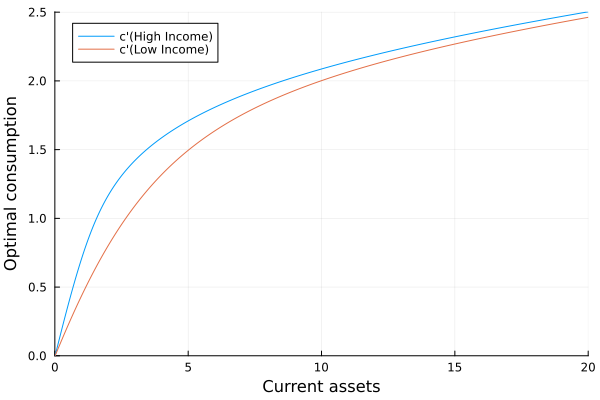
\includegraphics[width=10cm]{macro_hw4_code/consumption_policy_function3.png}\caption{Optimal Consumption Policy, $b=4$}\label{fig6}\end{figure}\newpage
	\item I constructed two helper functions -- one to find the stationary distribution of the Markov chain (this is standard, and I copied older code), and one to simulate the series of asset choices over time (for 250,000 periods). I solved the model for 100 values of $r$ between 0.00 and $1/\beta - 1 \approx 0.0204$, the maximum interest rate that would ensure that $(1+r)\beta \le 1$, and attained the aggregate (mean) assets for each of those interest rates. They are plotted in Figure~\ref{fig7}. As we would expect, savings are directly increasing in the interest rates. Annoyingly, we have divergence as we get close to $r = 0.02$ (specifically, at the 89th iteration, when $r = 0.01814058956916102$). This doesn't make a ton of sense, but it appears to be a consistent pattern. 
	\begin{figure}[H] \centering 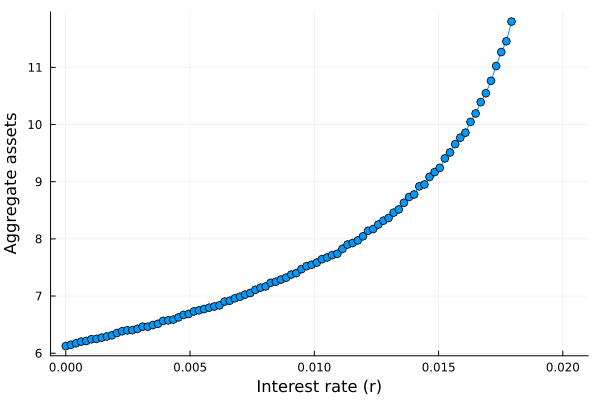
\includegraphics[width=10cm]{macro_hw4_code/aggregate_assets_vs_interest_rate.png}\caption{Aggregate Assets and Interest Rate}\label{fig7}\end{figure}
\end{enumerate}
As a reminder, the entirety of the code I used is below, in the \hyperref[sec:code]{Code Section}.


\newpage
\section*{Credit Markets and Economic Growth}

\begin{enumerate}
	\item Observe that if a worker with entrepreneurial ability $e_L = 0$ tried to operate their technology, they would attain output $f(e_L,\cdot,\cdot) = 0$, and attain 0 profit for any rental price. Thus, all of the low-ability individuals will solely supply labor in the competitive equilibrium. Additionally, we have directly that there are enough low-ability individuals that the high-ability individuals are incentivized to operate their technology rather than work -- so the profit from the rental price is strictly higher than the equilibrium wage. Conclusion will follow if we can show that the social planner will also prefer to assign all high-ability individuals to technology and all low-ability individuals to labor. We will use an argument similar to proving that a certain strategy is optimal in Game Theory -- by assuming that the social planner is following the same allocation, and proving that there are no profits (in fact, there are losses!) from deviation.\\\\ Assume that the social planner assigns all high-ability individuals to technology and all low-ability individuals to labor. First, it is plain to see that they will not improve by moving a low-ability individual to technology -- instead of producing marginal output of $f'_l(\cdot) > 0$, they will produce 0 as $e_L = 0$. Next, moving a high-ability individual to labor would have them produce marginal output $f'_l(\cdot)$ instead of $f'_k(\cdot)$. However, recall that in the competitive equilibrium we had that the high-ability individuals were incentivized to always operate their technology, meaning that $r > w$ (at their levels of ability and technology). Since competitive prices are the marginal outputs of each action, this implies that $f'_l(\cdot) < f'_k(\cdot)$, so moving a high-ability individual to labor would reduce output. \\\\Since we have shown that the social planner will choose the same production decisions as in the competitive equilibrium, they will attain the same output and the same consumption and investment decisions as well. Thus, we can compute the competitive equilibrium by solving the planner's problem.
	\item Observe that the production function is homogeneous of degree $1-\nu$ in $(k,l)$:\[f(e_i,\lambda k,\lambda l) = \lambda^{1-\nu} f(e_i,k,l) \forall \lambda > 0\]Since the production function is homogeneous, we can use a representative consumer for this economy. Formally, if we have a measure 1 of identical firms who each use $k_i,l_i$, where $\int_0^1 k_idi = K_i$ and $\int_0^1l_idi = \pi$, then we have that \[\int_0^1 f(e_i,k_i,l_i)di = e^\nu  \pi^{(1-\nu)(1-\alpha)} K_t^{\alpha(1-\nu)} = F(K_t)\]
	\item The social planner cares equally for the two agents. This means that total output will be divided so as to give the agents the same utility in each period. Thus, maximizing $c_H$ and $c_L$ is the same as maximizing aggregate consumption $C_t$. Formally, the planner maximizes \[\int_0^\infty e^{-\rho t} \barl \frac{c_H(t)^{1-\sigma}}{1-\sigma} + \pi \frac{c_L(t)^{1-\sigma}}{1-\sigma}\barr dt \]subject to\[\dot{K}(t) = F(K_t) - \delta K_t - (c_H - \pi c_L)\]so, since CRRA utility is increasing and monotonic, this is equivalent to just maximizing the sum $c_H + \pi c_L = C_t$.
	\item The social planner's (present-value) Hamiltonian is:\[\mathcal{H} = e^{-\rho t} \frac{C(t)^{1-\sigma}}{1-\sigma} + \lambda(t) \barl e^\nu  \pi^{(1-\nu)(1-\alpha)} K(t)^{\alpha(1-\nu)} - \delta K(t) - C(t)\barr\]which admits first order conditions \begin{align*} 0 &= e^{-\rho t} C(t)^{-\sigma} - \lambda(t) &&(C) \\ -\dot{\lambda}(t) &=\lambda(t) \parl \alpha(1-\nu) e^\nu \pi^{(1-\nu)(1-\alpha)} K(t)^{\alpha(1-\nu)-1} - \delta \parr &&(K) \\ \dot{K}(t) &= e^\nu  \pi^{(1-\nu)(1-\alpha)} K(t)^{\alpha(1-\nu)} - \delta K(t) - C(t) &&(\lambda) \end{align*} So differentiating the $C$ condition with respect to $t$, we get that\[\frac{\partial \lambda(t)}{\partial t} = \dot{\lambda}(t) = -\rho e^{-\rho t}C(t)^{-\sigma} - \sigma e^{-\rho t} C(t)^{-\sigma - 1} \dot{C}(t) \Longrightarrow \dot{\lambda}(t) = e^{-\rho t} C(t)^{-\sigma}\barl -\rho - \sigma \frac{\dot{C}(t)}{C(t)}\barr \] So, substituting into the $K$ condition, it becomes \[ -\rho + \sigma \frac{\dot{C}(t)}{C(t)}=  \alpha(1-\nu) e^\nu \pi^{(1-\nu)(1-\alpha)} K(t)^{\alpha(1-\nu)-1} - \delta \]and rearranging, we get\[\frac{\dot{C}(t)}{C(t)} = \frac{1}{\sigma}\barl \alpha(1-\nu) e^\nu \pi^{(1-\nu)(1-\alpha)} K(t)^{\alpha(1-\nu)-1} + \rho - \delta\barr\]which we can combine with the first order condition on $\lambda$\[\dot{K}(t) = F(K(t)) - \delta K(t) - C(t)\]These two ODEs, combined with the initial condition that $K(0) = K_0$, entirely characterize the paths for $C$ and $K$.
	\item If the low-ability agents start with the capital, the equilibrium dynamics will not change. To see why, observe that since using their capital is never profitable for the low-ability agents, they will simply choose labor and then rent their capital to the high-ability agents at a certain rate. To the social planner, this only affects the distribution of consumption between the types of agents, not the production or capital levels. Since we saw in part (3) that the social planner can solve only for aggregate consumption and attain the equilibrium, the distribution within that aggregated consumption won't affect anything. Thus, everything (except for the ratio of $c_H$ to $c_L$) will remain the same, including the dynamics of $C(t)$ and $K(t)$.
\end{enumerate}

\newpage
\section*{Code}\label{sec:code}

This code takes a long time to run, entirely because of the number of times the model is simulated for Question 5 in Part 1. If I had more time or ability, I could convergence time by using estimates from the previous interest rate. However, I am lazy. The code is:

\lstinputlisting[language=Julia]{macro_hw4_code/main.jl}



















\end{document}